\documentclass[10pt,a4paper]{article}

\usepackage[a4paper,margin=0.58in]{geometry}
\usepackage{graphicx}
\usepackage{booktabs}
\usepackage{url}

\setlength{\parskip}{0.35em}
\setlength{\parindent}{0pt}
\makeatletter
\setlength{\@fptop}{0pt}
\makeatother

\title{\vspace{-1.2cm}Robustness Analysis of Monocular Depth Estimation with Depth Anything V2}
\author{Deep Learning for Visual Computing - Assignment 3}
\date{\vspace{-0.4cm}}

\begin{document}
\maketitle
\vspace{-0.7cm}
\fontsize{9.2}{10.6}\selectfont

\section{What did we do?}

We experimented with monocular depth estimation, a computer vision task that predicts a dense depth map from a single RGB image. This is different from image classification or semantic segmentation because the model does not assign class labels; instead, it estimates the relative 3D structure of the scene.

We used Depth Anything V2, an open-source pretrained model for monocular depth estimation. Our goal was not to train a new model, but to study how a strong pretrained model behaves on realistic photos and on challenging visual cases. We built a small custom dataset from our own photos and teammate photos. The images were organized into eight categories: indoor, outdoor, mirror, glass/window, shiny metal, plain wall, very close object, and dark image. These categories were chosen because they contain common failure cases for monocular depth estimation, such as reflections, transparency, weak texture, low illumination, and extreme foreground objects.

We also compared three Depth Anything V2 model variants: Small, Base, and Large. For each model, we generated colored depth maps, side-by-side input/depth visualizations, and runtime measurements.

\section{Code source and modifications}

We downloaded the open-source implementation of Depth Anything V2 from the official GitHub repository:

\begin{center}
\url{https://github.com/DepthAnything/Depth-Anything-V2}
\end{center}

We did not modify the model architecture, pretrained checkpoints, or inference method. We chose V2 instead of V1 or V3 because V2 is a mature and widely used release with stable open-source code, pretrained checkpoints, and strong practical reproducibility. V1 is older, while V3 was newer and less established for our goal. Since the assignment emphasizes a reliable open-source experiment within limited time, V2 was the safest choice.

Our changes were limited to experiment automation and dataset organization:

\begin{itemize}
    \item We wrote a custom script, \texttt{run\_depth\_experiments.py}, to run inference on all images.
    \item We saved colored depth maps and side-by-side comparison images.
    \item We recorded per-image inference time and descriptive depth statistics in CSV files.
    \item We organized the custom photos into challenge categories for qualitative analysis.
\end{itemize}

\section{Problems while running the code}

We did not encounter major model-level problems when running inference on a CUDA GPU. The main practical issues were related to evaluation design rather than installation.

First, our own photos do not have ground-truth metric depth. Therefore, we cannot claim real numerical depth accuracy. We solved this by treating the experiment as a qualitative robustness study and a runtime comparison. The report discusses whether the predicted depth maps preserve plausible relative scene structure, but it does not claim metric accuracy.

Second, Depth Anything V2 outputs relative depth. The absolute numerical scale of the depth maps is not directly comparable between model variants. For this reason, we used the depth statistics only as descriptive information and used runtime as the main quantitative comparison.

Third, some low-light images were originally placed in the teammate's photo folder rather than in a separate \texttt{dark\_image} folder. We fixed this during dataset organization by labeling these images as dark/low-light examples in the metadata and analyzing them as part of the dark image category.

\section{Tests and results}

\subsection{Experimental setup}

We evaluated 28 photos in total. The categorized custom dataset contains 18 images across the eight challenge categories, and the teammate folder contains 13 additional photos, including low-light and indoor/outdoor scenes. The inference script was run with three Depth Anything V2 checkpoints:

\begin{table}[htbp]
\centering
\caption{Depth Anything V2 model variants used in the experiment.}
\begin{tabular}{lll}
\toprule
Model & Encoder & Device \\
\midrule
Small & \texttt{vits} & CUDA GPU \\
Base & \texttt{vitb} & CUDA GPU \\
Large & \texttt{vitl} & CUDA GPU \\
\bottomrule
\end{tabular}
\end{table}

This gives 84 inference runs in total. For each run, we saved a depth map, a side-by-side visualization, and runtime measurements.

\subsection{Runtime and model comparison}

Figure~\ref{fig:quantitative} summarizes the runtime comparison and a visual comparison of the three model variants on the same glass/window scene. Small and Base were very close in speed, while Large was slower. The three depth maps show broadly similar global structure; the larger model appears slightly more coherent around difficult transparent and distant regions, but this is a qualitative observation only.

\begin{table}[htbp]
\centering
\caption{Average inference time over 28 images.}
\begin{tabular}{lrr}
\toprule
Model & Encoder & Avg. inference time (sec/image) \\
\midrule
Small & \texttt{vits} & 0.229 \\
Base & \texttt{vitb} & 0.236 \\
Large & \texttt{vitl} & 0.425 \\
\bottomrule
\end{tabular}
\end{table}

\begin{figure}[htbp]
\centering
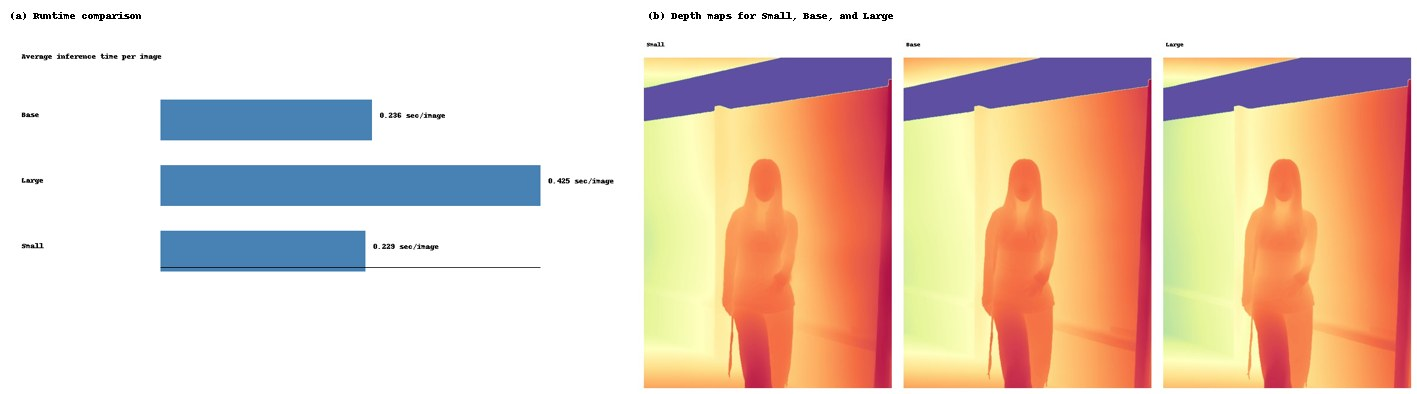
\includegraphics[width=0.92\linewidth]{figures/quantitative_model_summary.jpg}
\caption{Quantitative and qualitative model comparison: average inference time and depth maps for Small, Base, and Large.}
\label{fig:quantitative}
\end{figure}

\subsection{Qualitative category analysis}

Figure~\ref{fig:success} shows representative cases where the model produced plausible relative depth. Indoor and outdoor scenes were generally stable when the image contained perspective cues, object boundaries, and multiple visible depth layers. Very close foreground objects were usually detected as near, although they sometimes dominated the depth map.

\begin{figure}[htbp]
\centering
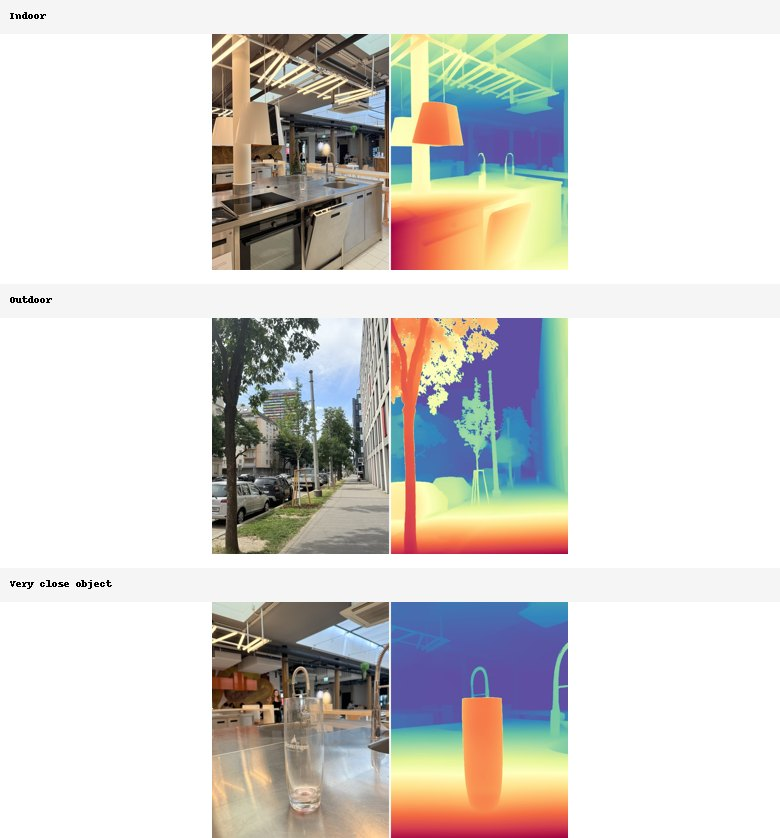
\includegraphics[width=0.82\linewidth]{figures/qualitative_success_cases.jpg}
\caption{Representative successful or mostly stable cases. Each panel shows the input image and the predicted colored depth map.}
\label{fig:success}
\end{figure}

Figure~\ref{fig:challenging} shows more difficult cases. Mirrors can be interpreted as real 3D space, glass/window scenes mix a transparent surface with objects behind it, shiny metal creates misleading reflections, plain walls provide weak texture, and dark images reduce visible boundaries.

\begin{figure}[htbp]
\centering
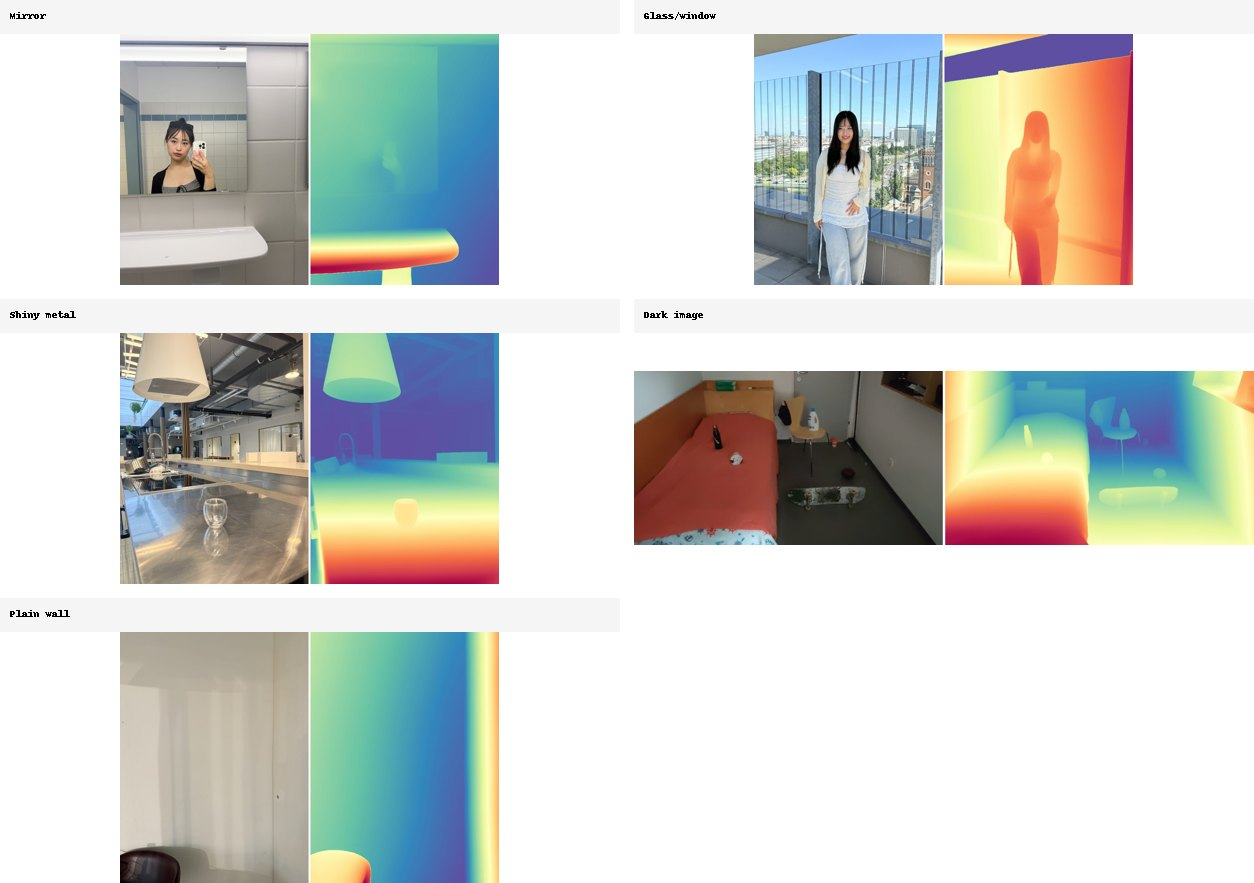
\includegraphics[width=0.88\linewidth]{figures/qualitative_challenging_cases.jpg}
\caption{Challenging examples: mirror reflection, glass/window ambiguity, shiny metal reflection, low-light image, and plain wall.}
\label{fig:challenging}
\end{figure}

\section{Discussion}

Overall, Depth Anything V2 produced visually plausible depth maps for many real-world scenes. The model was especially convincing when scenes contained strong perspective lines, foreground/background separation, and recognizable objects. The runtime comparison also showed that Small and Base were efficient, while Large was noticeably slower.

The most interesting failures appeared in images where monocular cues are physically ambiguous. Mirrors and transparent surfaces do not correspond cleanly to a single visible surface. Reflections on metal tables and glass can appear as real geometry. Plain walls and low-light images remove texture and edges, which are important cues for estimating depth from a single image. These results match the expected limitations of monocular depth estimation: the model can infer likely 3D structure from learned visual patterns, but it cannot directly observe true geometry.

The main limitation of our experiment is the lack of ground-truth depth. Therefore, our results should be interpreted as qualitative robustness analysis and runtime comparison, not as a benchmark of metric accuracy. A stronger future experiment would add an ordinal depth test with manually selected close/far point pairs, or use a benchmark dataset with annotated depth relations.

\section{Conclusion}

We successfully ran Depth Anything V2 on a custom set of real-world images and compared three model variants. The model worked well on normal indoor and outdoor scenes, but struggled more with mirrors, glass, reflections, textureless walls, and low-light images. This made the experiment useful for understanding both the strengths and limitations of monocular depth estimation.

\begin{thebibliography}{9}
\bibitem{depthanythingv2github}
Depth Anything V2 GitHub repository. \url{https://github.com/DepthAnything/Depth-Anything-V2}

\bibitem{depthanythingv2paper}
Depth Anything V2 paper. \url{https://arxiv.org/abs/2406.09414}
\end{thebibliography}

\end{document}
